%!TeX root = paper22-coord-ac-rl.tex
\newcommand{\figfactor}{0.45}
\begin{figure}[t!]
  \bigskip
  \begin{subfigure}[t]{\figfactor\textwidth}
    \centering
    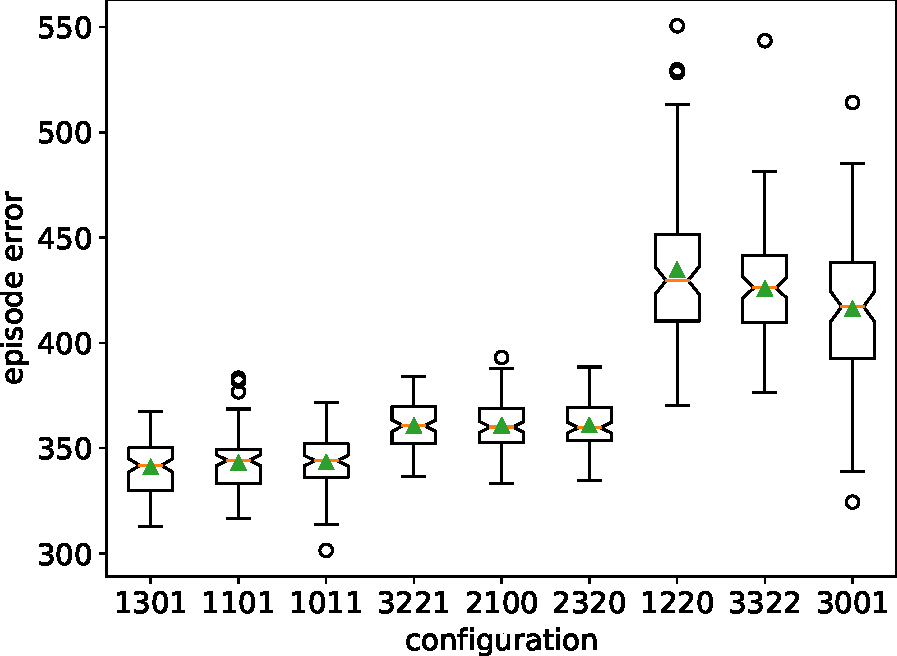
\includegraphics[width=\textwidth]{papers/coordination2022/img/box-all.pdf}
    \caption{Box plots of last $G_s$ episode.}
    \label{coordination2022:subfig:boxplot}
  \end{subfigure}  
  \hfill
  \begin{subfigure}[t]{\figfactor\textwidth}
    \centering
    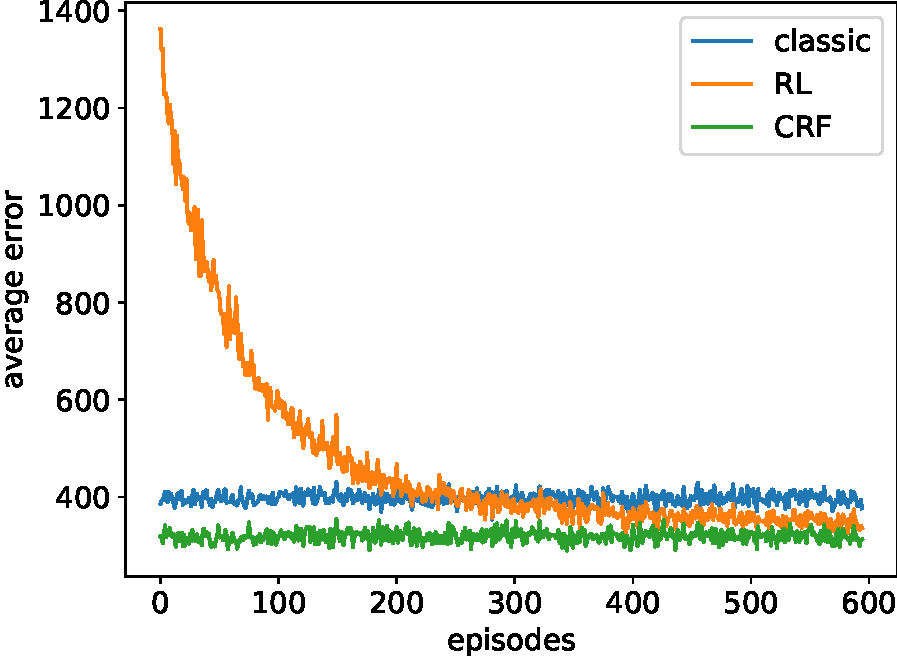
\includegraphics[width=\textwidth]{papers/coordination2022/img/mean-error-left.pdf}
    \caption{Learning progress of the best result.}
    \label{coordination2022:subfig:mean-error-over-episode}
  \end{subfigure}
  \bigskip
  
  \begin{subfigure}[t]{\figfactor\textwidth}
    \centering
    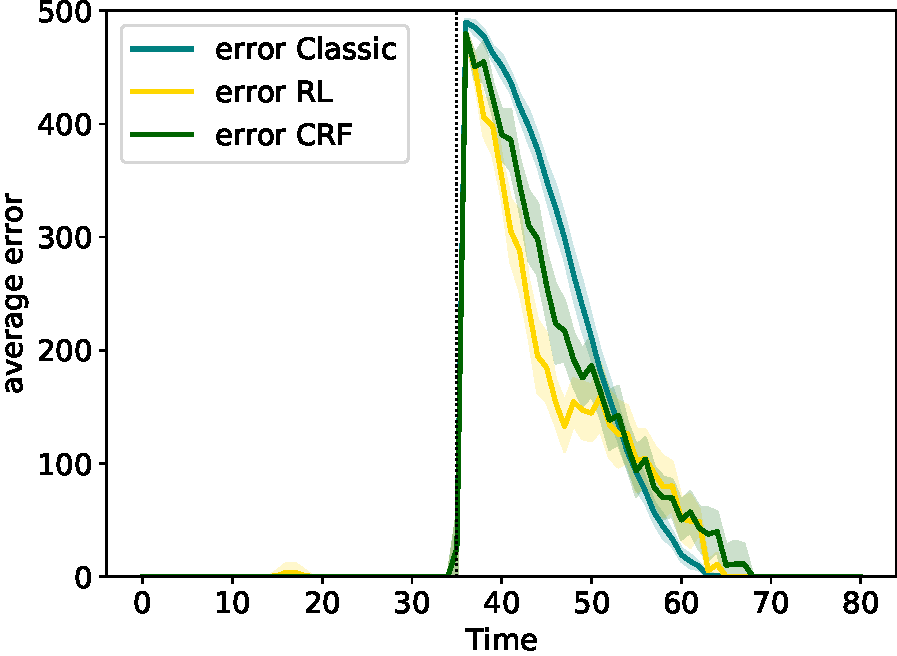
\includegraphics[width=\textwidth]{papers/coordination2022/img/error-few-nodes.pdf}
    \caption{Error evolution with 40 agents}
    \label{coordination2022:subfig:error-few}
  \end{subfigure}
  \hfill
  \begin{subfigure}[t]{\figfactor\textwidth}
    \centering
    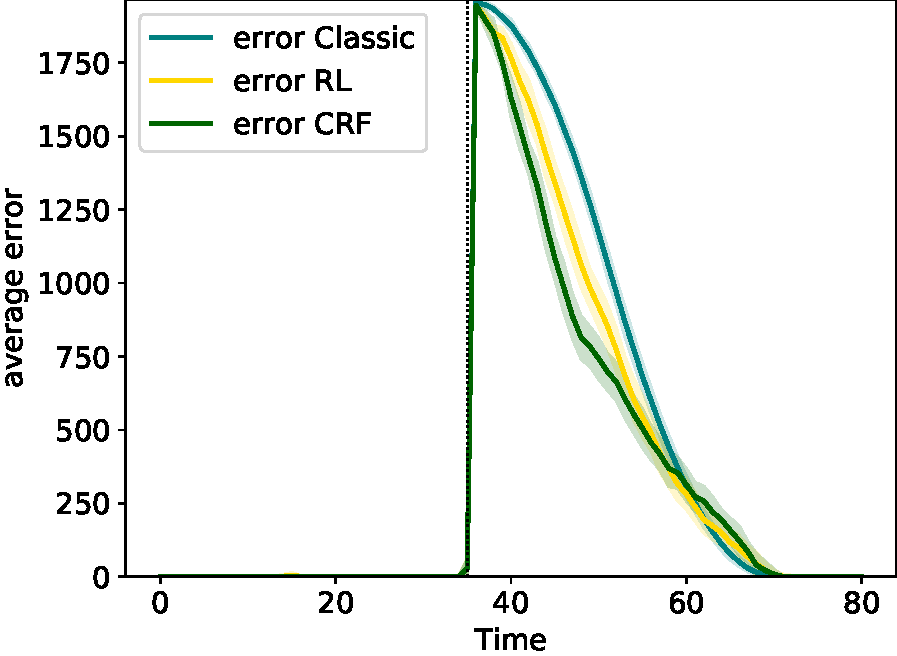
\includegraphics[width=\textwidth]{papers/coordination2022/img/error-many-nodes.pdf}
    \caption{Error evolution with 200 agents}
    \label{coordination2022:subfig:error-many}
  \end{subfigure}
  \bigskip
  
  \begin{subfigure}[t]{\figfactor\textwidth}
    \centering
    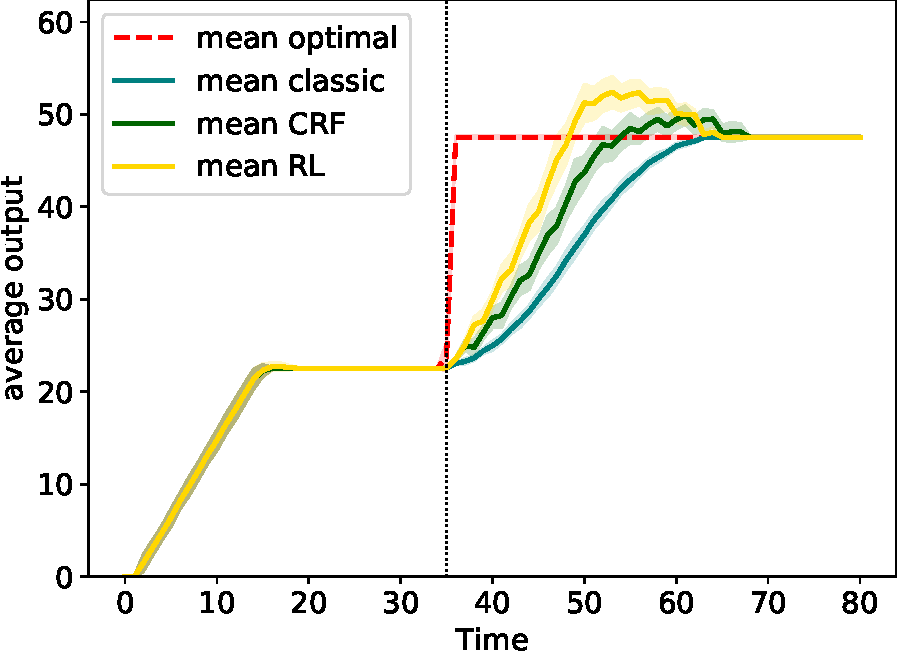
\includegraphics[width=\textwidth]{papers/coordination2022/img/output-few-nodes.pdf}
    \caption{Output evolution with 40 agents}
    \label{coordination2022:subfig:output-few}
  \end{subfigure}
  \hfill
  \begin{subfigure}[t]{\figfactor\textwidth}
    \centering
    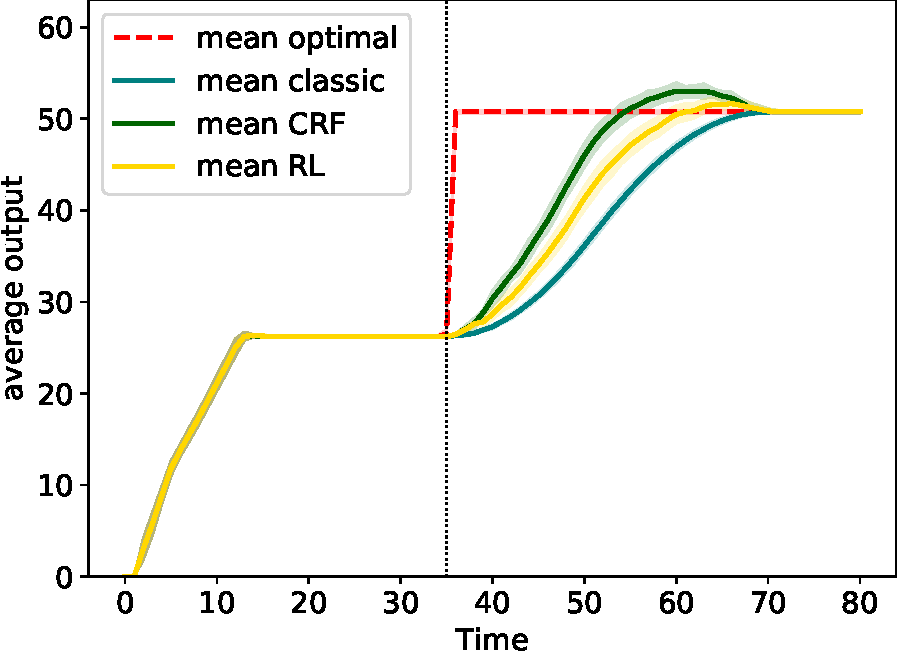
\includegraphics[width=\textwidth]{papers/coordination2022/img/output-many-nodes.pdf}
    \caption{Output evolution with 200 agents}
    \label{coordination2022:subfig:output-many}
  \end{subfigure}
  \caption{Performance of our \ac{rl}-based gradient algorithm with \lstinline|velocity| = 20.
  }
  \label{coordination2022:fig:eval}
\end{figure}